\chapter{Graph}

\section{Export CSV}
To export the measured data to a csv-file, the button ``Export CSV'' in the graph part of the graphical user interface, shown in figure \ref{fig:graph} has to be pushed. This opens the export dialog, shown in figure \ref{fig:exportcsv}, where the path and the file name can be chosen and experiments can be muted, if this is desired. To confirm the export of the measured data, the button ``OK'' has to be pushed.

\begin{figure}[!ht]
	\centering
		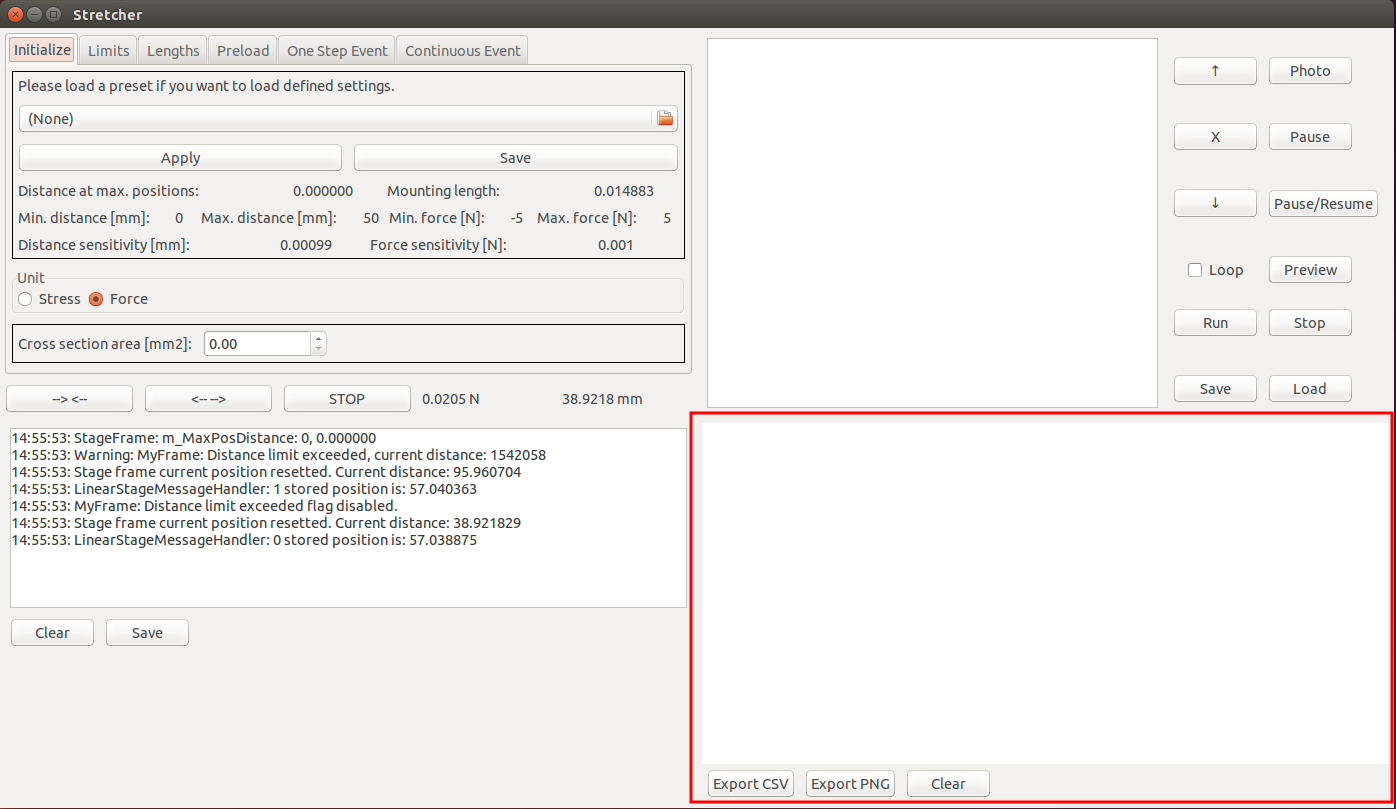
\includegraphics[width=1.0\textwidth]{images/Graph}
	\caption{Graph}
	\label{fig:graph}
\end{figure}

\begin{figure}[!ht]
	\centering
		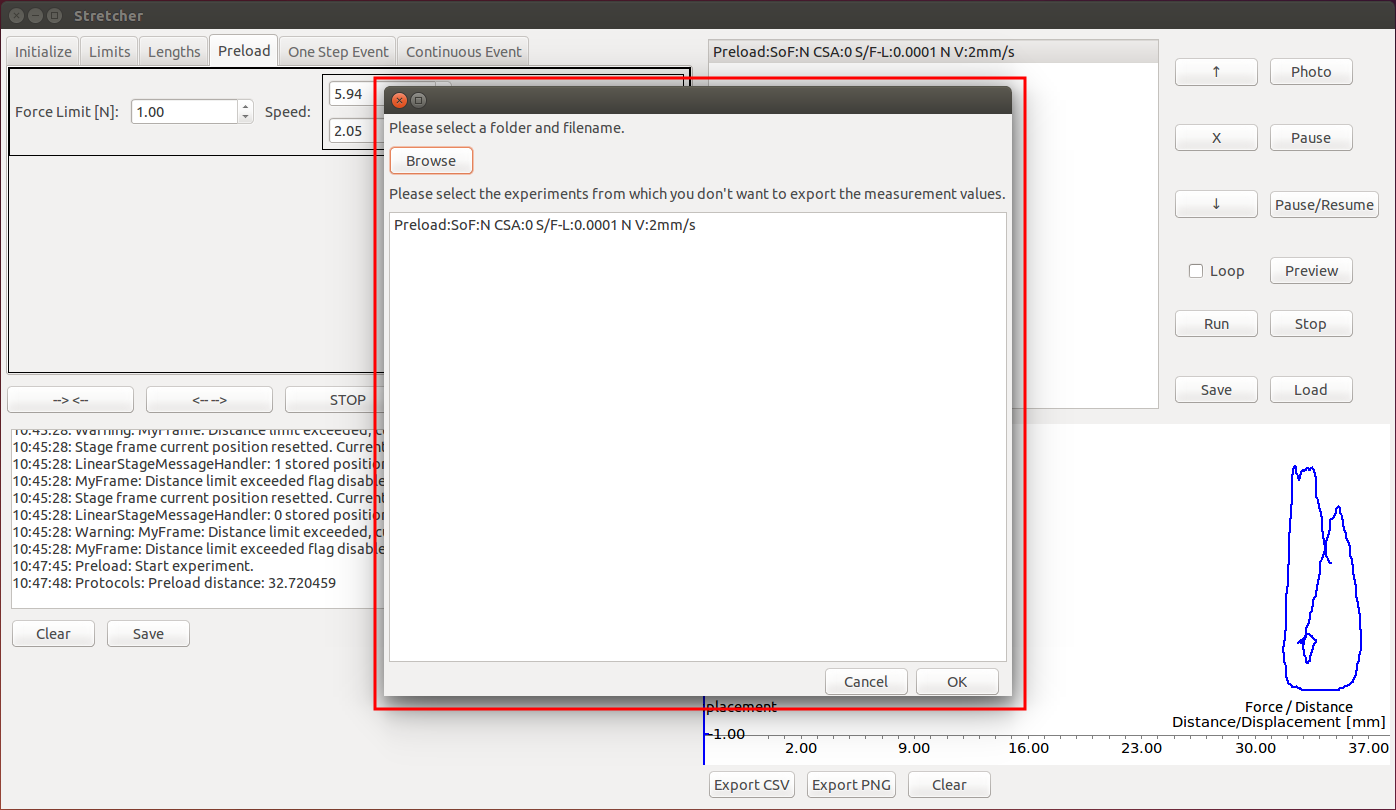
\includegraphics[width=1.0\textwidth]{images/ExportCSV}
	\caption{Export CSV}
	\label{fig:exportcsv}
\end{figure}

\section{Export PNG}
It is also possible to export the graph as a png image. For this the button ``Export PNG'' has to be pushed, and the path and a file name has to be chosen and then the export has to be confirmed by pushing the button ``OK''.